%!TEX root = ../../dissertation.tex
%%%%%%%%%%%%%%%%%%%%%%%%%%%%%%%%%%%%%%%%%%%%%%%%%%%%%%%%%%%%%%%%%%%%%%%%%%%%%%%%
\section{Influences of the Existing Stack}
\label{c5:sec:stack-influences}

This section briefly covers the existing Web protocol stack, which is also used for reliable streaming, in relation to mobile networks and streaming, new protocols and how they might influence the stack, and also discusses \gls{TCP} more closely as an example. Beneficial interactions between the stack's layers are presented in a final part.

Superficially, not much has changed in the Web's protocol stack. There is still \gls{IP}, \gls{TCP}, and \gls{HTTP} forming effectively the same stack since the development of HTTP/0.9 in 1991. And this seems hard to change. Especially the transport layer is fixed to \gls{UDP} and \gls{TCP}, everything else will probably get rejected, altered or even dropped by one of the numerous middleboxes, such as \glspl{NAT}, or forced ``traffic optimization'' transparent proxies, all of which are prevalent in mobile networks \cite{sigcomm11middleboxes}. As a side note, this adds another layer of state kept in the network. A fact that was already discussed as being highly problematic and capable of inducing load in the core network in Chapter~\ref{chap:mobilenets}.

Each protocol, representing a layer in the stack, characteristically contributes to influencing data transmissions and varies in its degree of impact on the network as well as the intended goal of the transmission (e.g., streaming and watching a video).

\begin{figure}[htb]
	\centering
	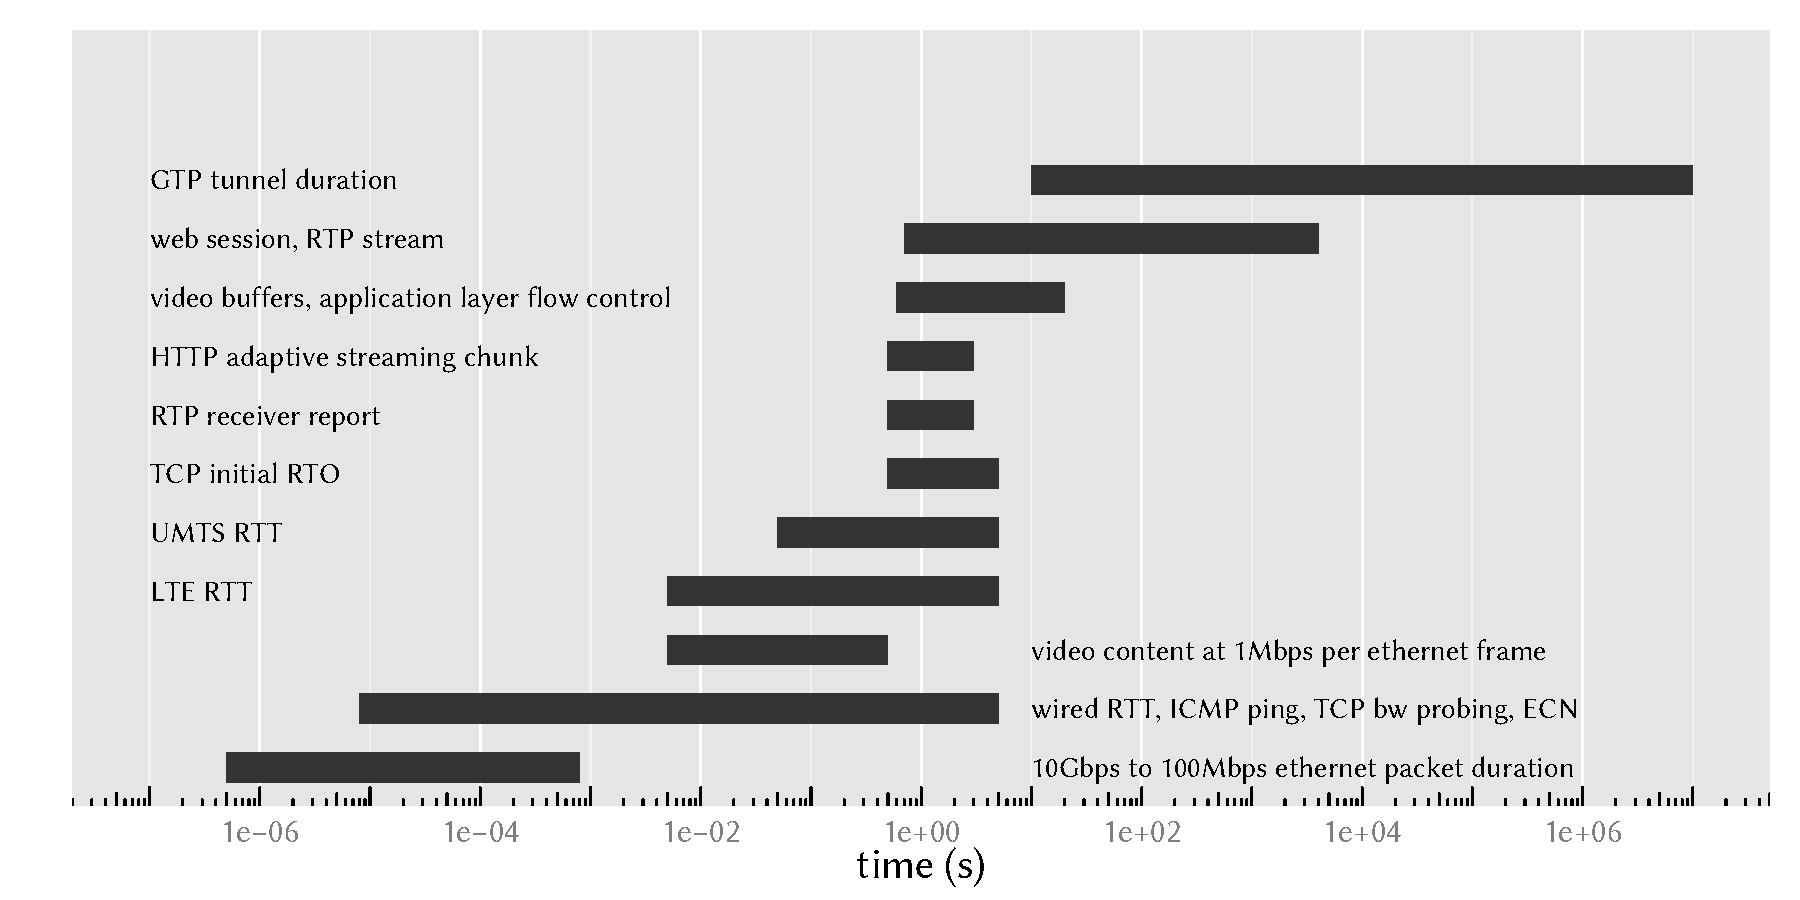
\includegraphics[width=1.0\textwidth]{images/layer-timescales.pdf}
	\caption{Approximate discernible time scales the networking stack protocols operate on in each layer.}
\label{c5:fig:timescales}
\end{figure}

Associated with each layer, and with the actual application running on top of the stack as well, are different timing constraints or time constants of control. Figure~\ref{c5:fig:timescales} overviews the approximate time scales on which activities take place, spanning a remarkable range of twelve orders of magnitude. Complexity is introduced by stacking multiple layers on top of each another, with many layers bringing along their own notion of control and feedback loops. Functionality might be duplicated across different layers, e.g., flow control in the application and on transport layer, leading to nested control loops, which might be coupled due to the timing constraints.

From the application layer end-to-end perspective the mobile network protocols seem to simply increase the depths of the protocol stack. Still, there are effects present that are specific to wireless access and differentiate mobile networks from a fixed and ``dumb'' bit pipe.

Typical effects of wireless connectivity relating to physical phenomena like fading and interference can be observed. Interruptions in the radio link are a major source of packet loss and spiking delay.The overall delay in a mobile network is also strongly dependent on the mobile network technology in use and has considerably decreased over the last few specification evolutions, even in the core network. This was investigated in \cite{laner2011dissecting3gdelay}. But the \gls{RAB} and \gls{gtp} tunnel setup --- as previously described in Section~\ref{c4:sec:3gpparchitecture} --- is even with the latest iteration of specifications sufficiently lengthy to be measurable and influences packet delay on initiating connections as was observed in \cite{arlos2010packetsizedelayinfluence}.

To save radio and network resources devices usually have to quickly release their alloted radio resource slots causing additional delay for applications during connection reestablishment. Moreover, mobile networks offer many control options and parameters that can further influence any of the upper layers. Mobile devices have the tendency to be somewhat sensitive to some of these changes. For example, the authors of \cite{sigcomm11middleboxes} show the impact from protocol manipulations conducted by middleboxes. 

Comparing all these factors to wired protocols such as 802.3 Ethernet it is clear that much more can happen in the mobile stack. Today Ethernet is a point-to-point protocol, transmission delay depends only on very few predictable factors, such as the distance. Wired access is typically not conducted solely through Ethernet, but with access technologies such as \gls{DSL} using \gls{PPPoE} or cable with \gls{DOCSIS}. While they also add more layers to wired access, they should be by far less influencing than the mobile stack. The latter has to additionally manage mobility and the shared wireless radio medium with protocols such as \gls{RLC} and \gls{RRC}.

A further detail can be found in the interaction between mobile network frame sizes and the \gls{IP} \gls{MTU}. Usually \gls{IP} adapts its packet size to the shortest frame size of all the link layer links in the path using \gls{PMTU} discovery as described in \cite{rfc1191}. Unfortunately, this can not work in \gls{3G} mobile networks, user packets are transparently fragmented by the radio protocols to fit into the transmission slots alloted to the device. For example, a \gls{GPRS} transmission slot has a length of only \SI{576.9}{\micro\second} carrying just \SI{114}{\bit}. And in \gls{UMTS} \SI{40}{\byte} of payload are typically carried in each \gls{RLC} frame (with optional header compression in the \gls{PDCP} layer).

This fragmentation is another source of an undesired interaction between \gls{3G}'s link layer and everything above and including the network layer, potentially fragmenting packets over a long period and thereby causing delay.

In a neutral network, all packets are treated the same and should be subject to the same \gls{RTT} influencing sources. However, delays in the delivery of certain data to the upper layers can occur due to certain protocol features, such as \gls{TCP} retransmissions. After being detected through timers or duplicate acknowledgments any lost packet is automatically retransmitted by the sender. Therefore, loss from the lower layers is hidden from the application layer at the cost of delay variations and probably increased overall delay. The increase in delay is especially noteworthy in a \gls{3G} cellular network with its notion of link layer \gls{ARQ} and mobility. With the latter concept, transmissions originally running through one radio tower have to be moved to a new tower after a handover, even if the handover period was lengthy. These two combined can be the source of very high delay, reaching seconds or even hundreds of seconds, when moving quickly between coverage areas (e.g., in a car or train). 
This also causes bad interactions with \gls{TCP}, as these long-delayed segments are thought to be lost and subsequently retransmitted, resulting in an even further increase of delay and delay jitter.

Another undesirable influence factor is caused by each packet buffer in the transmission's path. The effect occurs if the size of the buffer is not chosen carefully and the following link is a bottleneck link. Additionally, memory is very cheap, so hardware vendors tend to plug in as much as they can. Packets may be kept unnecessarily long in these buffers, heavily increasing packet delay and diminishing \gls{TCP}'s ability to adapt itself to its fair share with the congestion control mechanisms~\cite{jacobson1988congestion,scharf2011comparison}. These mechanisms rely on feedback from the network by inducing packet loss which does not happen in a timely manner in case of large buffers. This phenomenon has been dubbed \textit{Bufferbloat}, and can induce latency as high as several seconds~\cite{gettys2011bufferbloat,groenewegen2011detecting}. And this is in addition to the latency in mobile networks that is already high and unreliable to begin with.

Buffers are necessary to compensate for short-term variations in the traffic load and avoid loss in these situations. A popular countermeasure are \gls{AQM} methods that control the size of the buffer and selectively drop packets if necessary. Although, most of these are never widely used because of configuration issues. One particular algorithm stands out that is becoming increasingly popular: CoDel~\cite{Nichols:2012:CQD:2209249.2209264, nichols2014codel}.

CoDel measures the time it takes for a packet to pass through a buffer and begins dropping packets once a certain limit has been surpassed in a predefined interval. This and other similar mechanisms that control queue delay and not its size have begun to appear and be used in several places, e.g., in the Linux Kernel.

Up to the point of the transport layer the layers are pretty well defined, with only a few select protocols to choose from, all with well known influence factors on the mobile network. The application layer has a different notion, though. Adhering to the end-to-end design principles most innovation (and therefore change) will take place at the utmost ends, i.e., the application layer. Even when only considering video streaming applications the protocol variations are countless as the overview and classification in Section~\ref{c3:sec:background} demonstrated. 

In streaming over mobile networks the video buffer size has to be in the range of seconds to compensate for most eventualities as seen in Figure~\ref{c5:fig:timescales}. And every streaming protocol has slightly different time scales and feedback loops.

As is the case in any best-effort network no bandwidth, latency, or loss guarantees can be given. The available bandwidth might get unexpectedly smaller resulting in a quickly draining video buffer if it was chosen too small. Then again, given sufficient bandwidth stability or at least predictability, buffer sizes could also be kept at a bare minimum, thereby enabling or improving real-time interactivity. In addition to a fitting choice of the buffering and playback strategies the choice of segment length and quality levels in adaptive streaming also plays an influential role in mobile networks. Most of these factors were discussed in Chapter~\ref{chap:streaming}.

In layered network models individual functions are strictly separated and stacked on top of each other with well-defined \glspl{API} connecting them. To achieve complete separation without cross-influences, the feedback and control loops of each layer also would need to operate on completely disjoint time scales. Looking again at Figure~\ref{c5:fig:timescales}, it can be seen that this notion is only partly supported and the loops of adjacent layers typically overlap somewhat. Protocols and implementations need to be aware of this circumstance and able to handle cross-layer influences.


%%%%%%%%%%%%%%%%%%%%%%%%%%%%%%%%%%%%%%%%%%%%%%%%%%%%%%%%%%%%%%%%%%%%%%%%%%%%%%%%
\section{Recent and Upcoming Protocols}

Protocol development has not stopped in recent years. On the contrary, especially in the application and transport layers some interesting changes are occurring. The following paragraph highlight some of the changes and their potential influence on or improvements to mobile streaming.

Beginning at the transport layer some alternative approaches to \gls{TCP} are available, as especially the retransmission reliability has proven to be problematic in mobile networks as discussed. Typically, \gls{TCP} is used regardless for two reasons: First, having congestion control is an absolute necessity to achieve an equal fair share bandwidth and avoid congestive collapse. If no congestion control is present on the transport layer it would need to be implemented in the application layer. This generates additional implementation work and simultaneously reduces portability and compatibility to other congestion control variants --- the term \textit{TCP friendliness} has been used for this in the literature. 

Second, due to many middleboxes simply dropping packets using any unrecognized protocol --- exempting \gls{UDP} and \gls{TCP} --- the transport layer protocol often can not be changed at will. New transport protocol approaches would need to layer themselves atop \gls{UDP} incurring additional overhead. These following three items are examples of such transport protocols, each created with different goals in mind:

\begin{itemize}
	\item \gls{DCCP}~\cite{rfc4340} extends \gls{UDP} with concepts for data flow and \gls{TCP}-compatible congestion control but omits a strict packet retransmission feature.

	\item The \gls{LEDBAT}~\cite{rfc6817} congestion control algorithm which is implemented, amongst others, in \gls{uTP}~\cite{bt2010utp}. Traffic using \gls{LEDBAT} is generally of high volume, high elasticity, and low priority, such as for example file sharing traffic. Data handled by this congestion control approach gets displaced by any other data if the algorithm detects an increase in the transmission buffer delay.

	\item \gls{QUIC}\footnote{\url{http://lwn.net/Articles/558826/} and \url{http://www.ietf.org/proceedings/88/slides/slides-88-tsvarea-10.pdf}} is a further experimental approach aimed at reducing sources of latency spikes which would occur in \gls{TCP}, such as retransmissions or the initial handshake. Some reliability is achieved through \gls{FEC} schemes if desired. Furthermore, a novel congestion control mechanism based on packet pacing, not through a traditional congestion window, and encryption by default are implemented. However, it is not intended as a production protocol but is rather a testbed for future mechanisms and modifications to existing protocols.
\end{itemize}
%
Especially \gls{DCCP} and \gls{QUIC} show some interesting prospects for mobile streaming through their omission of retransmissions, which is the source of most playback stalling in high latency and loss scenarios. This would return streaming players a degree of freedom which they had while using the unreliable \gls{rtp}. A playback strategy could now once again decide what to do in case of packet loss. The choice would be either to stall and wait for subsequent video data or drop some frames and continue the playback more rapidly.

In the wake of Edward Snowden's surveillance and man-in-the-middle reveals, the \gls{IETF} announced its position on these issues in \cite{rfc6973} suggesting that all future standardized protocols should consider surveillance issues and minimize or prevent any attempt on it. Ultimately, this might lead to a end-to-end \textit{crypto-by-default} Internet, with every protocol providing at least opportunistic encryption. The first signs are already visible in today's traffic mix, with many Websites only available through \acrshort{HTTPS} --- using \gls{TLS}~\cite{rfc5246} --- any more. Similarly, most e-mail providers have moved to \acrshort{IMAPS} and \acrshort{SMTPS}, even using new authentication and key exchange techniques like \gls{DANE}~\cite{rfc6698} which in turn relies on \gls{DNSSEC}~\cite{rfc4033} to authenticate the validity of \gls{DNS} entries. For example, the current draft version of \gls{HTTP}/2 --- which will be described in more detail shortly --- mandates the presence, albeit not the usage, of \gls{TLS} capabilities in both client and server. And even the connectionless \gls{UDP} can be secured using \gls{DTLS}~\cite{rfc6347}.

Usually, an additional intermediate layer is added through the encryption process, adding more timing interdependencies to the other layers. However, end-to-end encryption also diminishes the influence of most middleboxes as they are not able to alter the contents of the --- now encrypted --- segment any more. More and more Web streaming are also available through \gls{HTTPS}, which causes a large shift of the traffic mix to encrypted protocols. Even for \gls{rtp} encrypted variants, in the form of SRTP~\cite{rfc3711} and ZRTP~\cite{rfc6189} are available and are being commonly used for communication applications.

Moving on to the application layer, some interesting developments have occurred in the Web's stack and in its use of \gls{HTTP} which almost all reliable streaming methods facilitate.

The original HTTP/1.0 specification is from the year 1996 with only one update to HTTP/1.1 in 1999 thereafter. Since then, no changes have been made to the core protocol. However, the number of use cases facilitating \gls{HTTP} has increased significantly, bringing with them a lot of long-standing issues that were not though of initially.

The typical number of individual \gls{HTTP} requests for one Web page has steadily increased, reaching today about \numprint{100} objects.\footnote{\url{http://www.websiteoptimization.com/speed/tweak/average-web-page/} and \url{http://httparchive.org/trends.php} and \url{https://developers.google.com/speed/articles/web-metrics}} \gls{HTTP} deals with this through persistent connections and pipelining to avoid unnecessary connection establishment and request delays. Pipelining is however disabled in almost every client implementation as it suffers from head-of-line blocking. To circumvent this problem and increase retrieval speed, browsers have begun to open many parallel \gls{TCP} connections per site, invoking significant overhead and general fairness issues due to the large number of \gls{TCP} connections displacing other traffic. Segment-based reliable streaming applications faces similar issues, especially when more than one segment is to be retrieved simultaneously. In the worst case, this can add additional latency through the need to establish further connections.

Moreover, the Web's structure has changed in such a way that it is now common to push data to the clients to increase a Web page's interactivity. However, \gls{HTTP} is a simple client-initiated request-response protocol and pushing can only be emulated using techniques such as \textit{long polling} which imposes several restrictions and state overhead. Both these issues also affect reliable streaming with \gls{HTTP} to a certain degree. Streaming can benefit from a reduction of request latency as well as servers pushing adequate video segments at the correct time without the need for further requests.

To combat the situation and increase the protocol's interactivity along with it, several approaches are being developed. The first, WebSocket~\cite{rfc6455}, is a transport protocol on top of \gls{TCP} (or \gls{TLS}) that can be established through a regular \gls{HTTP} connection. It enables full-duplex communication between the two communication nodes. An additional \gls{W3C} \gls{API}~\cite{w3c2011websockets} enables simple usage in browsers with higher interactivity than plain \gls{HTTP}. It is also used to stream content to a browser.

The \acrshort{WebRTC} protocol suite\footnote{\url{http://www.webrtc.org/}}~\cite{webrtcdraft} even goes a step further and provides a complete stack for multimedia communication. It is intended to be used --- through the provided \gls{API} --- for direct browser-to-browser communication initiated by a central server-side Web page.

Both these techniques aim to enhance or sidestep \gls{HTTP}. But it is also desirable to improve the protocol itself for the aforementioned reasons. Therefore, in 2010 Google implemented a new experimental application protocol called SPDY as an alternative to \gls{HTTP} in its Chrome browser accompanied by a draft specification~\cite{google2011SPDYdef, google2010SPDYwp}. Every major browser and most Web servers now support SPDY, many Cloud and \gls{CDN} providers have it enabled.

SPDY uses the same port as \acrshort{HTTPS} (443) and mandates the use of \gls{TLS} as it also serves to negotiate the choice between \gls{HTTP} and SPDY.\@ Compared to \gls{HTTP} pipelining, SPDY provides full-duplex time-division multiplexing. After an initial request of a Web page, the server can anticipate any follow-up requests, push objects on additional streams with assigned priorities and therefore avoid additional request round trips.

All of the SPDY changes are aimed at reducing the number of established \gls{TCP} connections for a Web site retrieval, ideally down to one, and reduce the overall latency of the object transmissions. Evaluations in \cite{google2010SPDYwp} suggest an average Web page load time reduction of \SI{29}{\percent}. The gains for networks with high latency, e.g., mobile networks, the gain could be even higher as several round trips are avoided.

Some of the benefits are also applicable to reliable streaming, with video segments being able to be pushed from the server. Conjoined with \gls{SVC}, SPDY could multiplex the different video layers in one connection, with the highest priority assigned to the base layer.

The SPDY draft was later picked up by the \gls{IETF} Httpbis working group as an initial basis basis for the \gls{HTTP}/2 specification~\cite{http20draft} currently being finalized as of mid 2014. It follows the SPDY specs rather closely, with the only major difference being the use of \gls{TLS}. Its usage is not mandated anymore, merely its presence and, if used, the application of strong and ephemeral cipher suites.

In fact, Netflix, one of the largest commercial video streaming providers, already utilizes the features of the latest \gls{HTTP}/2 draft in its service. For example, segments are pushed by the server using \gls{HTTP}/2 multiplexing and are displayed as \gls{HTML}5 video.


%%%%%%%%%%%%%%%%%%%%%%%%%%%%%%%%%%%%%%%%%%%%%%%%%%%%%%%%%%%%%%%%%%%%%%%%%%%%%%%%
\section{Additional TCP Changes}

In addition to the previously described new transport protocols under development aiming to replace and surpass \gls{TCP}, \gls{TCP} itself is not as static as it may seem. While the basic wire frame and data interchange format has already been defined in 1981 in \cite{rfc793}, much of the specific behavior is free to be experimented with by further specifications and implementations. The most prominent example is the congestion control mechanism where every operating system takes hugely different approaches.


\begin{table}[htbp]
\caption{Assorted list of some select network stack changes in the Linux kernel that alter \acrshort{TCP}'s transmission behavior.}
\label{c5:tab:linux-stack-changes}
	\begin{tabu}{X[1.4]X[0.6]X[0.4]X[0.7]}
	\toprule
	\textbf{Change} & \textbf{Related Work} & \textbf{Kernel} & \textbf{Date} \\
	\midrule
	BIC as default congestion avoidance algorithm (from Reno) & & 2.6.8 & August 2004 \\
	CUBIC as default congestion avoidance algorithm & \cite{ha2008cubic} & 2.6.19 & November 2006 \\
	New \gls{TCP} Slow Start: HyStart & \cite{Ha20112092} & 2.6.29 & March 2009 \\
	Multipath \gls{TCP} & \cite{rfc6824} & external & 2011 \\
	\gls{TCP} User Timeout & \cite{rfc5482} & 2.6.37 & January 2011 \\
	Initial Receive Window \SI{10}{MSS} & \cite{rfc6928} & 2.6.38 & March 2011 \\
	Initial Congestion Window \SI{10}{MSS} & \cite{rfc6928} & 2.6.39 & May 2011 \\
	\SI{1}{\second} initial RTO (from \SI{3}{\second}) & \cite{rfc6298} & 3.1 & October 2011 \\
	Changes to sstresh and CWND bevahior & \cite{rfc5681} & 3.1 & October 2011 \\ % details: https://git.kernel.org/cgit/linux/kernel/git/torvalds/linux.git/commit/?id=9ad7c049f0f79c418e293b1b68cf10d68f54fcdb
	\gls{TCP} Proportional Rate Reduction & \cite{rfc6937} & 3.2 & January 2012 \\
	Byte queue limits and \gls{TCP} buffer limits &  & 3.3 & March 2012 \\ % https://lwn.net/Articles/454390/
	CoDel \acrshort{AQM} & \cite{nichols2014codel} & 3.5 & July 2012 \\
	\gls{TCP} Early Retransmit & \cite{rfc5827} & 3.5 & July 2012 \\
	\gls{TCP} small queues & & 3.6 & September 2012 \\ %http://lwn.net/Articles/507065/
	\gls{TCP} Fast Open (client side) & \cite{cheng2014tcptfo} & 3.6 & September 2012 \\
	\gls{TCP} Fast Open (server side) & & 3.7 & December 2012 \\
	\gls{TCP} tail loss probe & & 3.10 & June 2013 \\ % http://tools.ietf.org/html/draft-dukkipati-tcpm-tcp-loss-probe-01
	\gls{TCP} Forward RTO-Recovery & \cite{rfc5682} & 3.10 & June 2013 \\
	Low latency network polling & & 3.11 & September 2013 \\ %http://lwn.net/Articles/551284/ and http://www.linuxplumbersconf.org/2012/wp-content/uploads/2012/09/2012-lpc-Low-Latency-Sockets-slides-brandeburg.pdf
	Improved RTO calculation and handling of reordering & & 3.12 & November 2013 \\ % https://git.kernel.org/cgit/linux/kernel/git/torvalds/linux.git/commit/?id=0f7cc9a3c2bd89b15720dbf358e9b9e62af27126 and https://git.kernel.org/cgit/linux/kernel/git/torvalds/linux.git/commit/?id=ed08495c31bb991de636d2488abaa50b39f2ff4a
	\gls{TCP} Fast Open enabled by default & & 3.13 & January 2014 \\
	\gls{TCP} auto corking & & 3.14 & March 2014 \\ % https://git.kernel.org/cgit/linux/kernel/git/torvalds/linux.git/commit/?id=f54b311142a92ea2e42598e347b84e1655caf8e3
	PIE \acrshort{AQM} & & 3.14 & March 2014 \\ % http://tools.ietf.org/html/draft-pan-aqm-pie-01 and https://git.kernel.org/cgit/linux/kernel/git/torvalds/linux.git/commit/?id=d4b36210c2e6ecef0ce52fb6c18c51144f5c2d88
	\gls{TCP} Fast Open over IPv6 & & 3.16 & 2014 \\
	LISP & \cite{rfc6830} & 3.16 & 2014 \\
	\bottomrule
	\end{tabu}
\end{table}

Every one of these changes can have unforeseen repercussions or benefits for the application layer. The following paragraphs investigate some of the changes in the last few years and their implications.  Instead of implicitly exploring specific mechanism choices of closed source \glspl{os} and tracking their changes over the years, which would be extremely difficult, the \gls{TCP} implementation in the Linux kernel is taken as an example. The changes can be easily tracked by crawling through the patch sets and their commit logs of every kernel version. Sites like \url{http://kernelnewbies.org/} and \url{http://lwn.net/} simplify this process even more. Table~\ref{c5:tab:linux-stack-changes} depicts such an attempt to track the major changes affecting \gls{TCP} in the kernel.

Most of the changes plainly aim at reducing the number of required round trip times and increase the overall throughput while still maintaining fairness. This includes both small and larger changes, some of the more recent are:

\begin{itemize}
	\item The \gls{TCP} congestion window defines the maximum amount of data that can be transmit without having received any acknowledgments for the data. It is the central knob for all congestion control mechanisms.

	The initial window size was increased multiple times in the past --- from initially one segment, to three, and now to ten segments~\cite{rfc6928} ---  with the intent to accommodate for the increase in transmission bandwidth and higher expected traffic volume. With a ten segment window small \gls{HTTP} objects can be transferred without any ACK round trips reducing the average Web page load time. The initial window is also important for determining the achievable throughput in segmented streaming as the congestion window is often reset in the idle phase between segments.

	\item Another \gls{TCP} round trip can be saved by using the initial handshake itself for data transmission. \gls{TCP} Fast Open~\cite{cheng2014tcptfo} implements this and is again thought to reduce Web page load times.

	\item While the retransmission timeout is calculated through \gls{RTT} measurements, it is initially set to \SI{3}{\second}. This could add a high amount of delay if packets are lost during the handshake at the beginning of a connection. Implementations following RFC~\cite{rfc6298} set the default value to \SI{1}{\second} which may benefit especially mobile networks.

	\item The classic congestion avoidance algorithms do not work very well with networks with a large \gls{BDP} as the congestion window scaling entirely depends on the \gls{RTT}. Newer approaches reduce this dependence while also departing from the traditional linear growth congestion avoidance phase. Some of the congestion avoidance in use in today's \glspl{os} are 

	\begin{itemize}
		\item Reno~\cite{rfc5681}
		\item New Reno~\cite{rfc6582}
		\item Vegas~\cite{Brakmo:1994:TVN:190809.190317}
		\item Compound~\cite{song2006compound} (as an option in recent Windows versions)
		\item CUBIC~\cite{ha2008cubic} (default in Linux)
	\end{itemize}
\end{itemize}


All of these changes should serve to demonstrate the flux \gls{TCP} is in. It is constantly being adapted to current network and application needs. However, no adaptation or assumption as to specific applications are made on the transport layer. These kind of modifications can only be made on an end-to-end basis, i.e., at the application layer (cf.\ also the arguments in \cite{saltzer1984end2end}). All lower layers must be application-neutral as they could harm other application layer protocols.

This is contrary to the claims that the Internet is ossified and cannot accommodate any new applications any more (confer for example in \cite{turner2005diversifying}). Rather, \gls{IP} and \gls{TCP} serve as the undiscriminating common carrier of every type of data at the bottleneck of the Internet's protocol hourglass model.

It also demonstrates the difficulties and large optimization space reliable streaming has to deal with. Finding the correct combination of protocols for every layer, parameters for these protocols, and playback strategies for every user scenario is a very complex task and needs proper tools to ease this.


%\todo{add some concluding remarks on the adaptivity of TCP and the so-called hourglass model/ossified network that does not permit any changes at the hourglass's bottleneck (IP and TCP); mention again the correlations between the layers to lead over to the cross-layer section}

%Multipath TCP MPTCP~\cite{rfc6824}!
%Slow Start~\cite{rfc5681}
% HyStart~\cite{Ha20112092}


% http://etutorials.org/Mobile+devices/gprs+mobile+internet/Chapter+1+Introduction+to+the+GSM+System/Radio+Interface/
% http://books.google.at/books?id=Vk9AmYz7TfoC&pg=PA184&lpg=PA184&dq=umts+pdu+size&source=bl&ots=jeO-rpM8HK&sig=NB2FAB37YcdyujYUt_kaHYwLEOE&hl=en&sa=X&ei=KjCxU6C-FKip0AXh94GQDw&redir_esc=y#v=onepage&q=umts%20pdu%20size&f=false


%%%%%%%%%%%%%%%
%% unused

%Characteristics of UDP packet loss: Effect of tcp traffic \cite{sawashima97characteristics}


% CoDel:
%  Head drop not tail drop
%  Queues only as shock absorbers
%  What matters is the delay within a flow
%  CoDel measures minimal packet pass through time in the local device buffer during a defined interval
%  If minimum gets too high, too much buffering is happening
%  If delay value does not once fall below a target in the interval CoDel will start dropping packets
% 	Signals congestion and hopefully reduces source rate
% 	If stays above target, progressively more packets are dropped
% 	Target: 5ms; interval: 100ms, based on simulation results
%  Can be enabled in Linux since 3.5, but many NIC drivers do not support it yet
%  Every buffer along the path influences transmission
% 	Most impact on the node before the bottleneck
% 	Cell towers, dsl/cable modems, ...

%but successful protocols develop de-facto; de jure much harder (see \gls{3G})


%protocols without retransmission feature (lost packets are not relevant and cause head-of-line blocking) but still with the all-important congestion control + TLS
%inherits new TCP features such as TFO, snap start, ...
%congestion control not through CWND but through packet pacing
%includes stream multiplexing and TLS-like crypto by default


% Multiplexing/Streams:
%  Control and Data Frames, with header compression
%  Stream interleaving/multiplexing or cancellation

%  Stream priorities (8 levels)
% 	Prefer essential resources over others (images)
% 	Prefer data with earlier deadlines? (E.g. load next few video streams immediately while already requesting more)

%  HTTP/1.1 syntax still viable as a layer on top of SPDY


% Evaluations:
% 	Average reduction in page load time: ~29\%; 27\% - 60\%
% 	Strongly dependent on connection, server environment
% 	HTTP/1.1 optimization (resources split on multiple domains) prevents SPDY multiplexing gains
%  SPDY could be more susceptible to packet loss and TCP congestion window downscaling
% 	Only one connection used compared to multiple HTTP/1.1


% IW10: better response time, still fair \cite{rfc6928}
% An argument for increasing \gls{TCP}'s initial congestion window \cite{dukkipati2010argument}
% IW3, IW10  Initial window size (IW10, ...)
%  TCP Congestion Window
% 	Maximal number of packets in flight
% –	Scaling through congestion control and avoidance algorithms
%  Initial Value
% 	1 (RFC1122, RFC2001)
% 	4000 Bytes (~ 3 packets) (RFC2414, RFC3390, ~2002)
% 	IETF proposal: IW10 
%  Rationale
% 	HTTP request for small websites using new TCP connection
% 	Transmit whole site in one RTT instead of multiple
% 	Reduces average latency
% 		Evaluation: ~10\% page load reduction on typical web pages
% 	High IW values already used by many CDNs


%Also look at ``An in-depth study of LTE: effect of network protocol and application behavior on performance'' \cite{Huang:2013:ISL:2486001.2486006}

% TCP Fast Open~\cite{cheng2014tcptfo}
%  Small server-side application adaptation required
%  Send data in the SYN and SYNACK packets
% 	Deliver it immediately to the application
% 	Only allowed for subsequent connections, requires additional security cookie (specific to client-server IP pair)
%  Saves one initial RTT
%  4\% to 41\% popular web page load time improvement

% OS-dependent receive window scaling behavior
% OS-dependent choice of packet size
% OS-dependent initial congestion window 3-10 packets
% \gls{TCP} changes (Fast Open, IW10, ...; any relationship to streaming? maybe faster)
%SACK or no SACK, CUBIC, ...

%Nagle's Algorithm~\cite{rfc896} delaying and aggregating small data packets





% TCP Early Retransmit \cite{rfc5827}
%  TCP loss recovery (not using SACK) triggers on
% 	Timeout (may be lengthy, ~RTT, min 1s)
% 	Triple duplicate ACK (fast retransmit)
% 		If CWND is small, TCP may not be able to get enough DUPACKs to trigger
% 		Reduce DUPACK threshold for these connections
% 	Less robust to segment reordering
%  Reduces average latency for narrow and lossy connections


% Proportional Rate Reduction PRR (RFC 6937 \cite{rfc6937} vs. rfc 3517)
%  TCP behavior on packet loss in the past
% 	RFC 3517: reduce CWND to half
% 		Must first ACK large portion of the data still in flight before transmitting again
% 	Linux: ``Rate halving''; Reduce CWND by 1 on every ACK until CWND/2
% 		Can still send data during recovery
%  Google IETF Proposal (Linux 3.2, January 2012): PRR
% 	Reduce timeouts by avoiding excessive window reductions
% 	Converge to cwnd chosen by congestion control by the end of recovery
% 	Can improve packet loss recovery time and average latency


%Congestion Avoidance algorithm ((New Reno~\cite{rfc6582}, Vegas~\cite{Brakmo:1994:TVN:190809.190317}, Compound~\cite{song2006compound}, BIC, CUBIC~\cite{ha2008cubic}; all w or w/o SACK)
%general basic tcp congestion control in \cite{rfc5681}, describing Reno